\documentclass[uplatex,11pt,dvipdfmx,aspectratio=169,unicode,t]{beamer}

% 和文用
\usepackage[utf8]{inputenc}
\usepackage{bxdpx-beamer}
\usepackage{pxjahyper}
\usepackage{minijs} % 和文用
%\usefonttheme{serif}
\renewcommand{\kanjifamilydefault}{\gtdefault} % 和文用
\usepackage{mathtools}
\usepackage{amssymb}
\usepackage{epic,eepic}
\usepackage{color}
\usepackage{caption}
\usepackage{amsmath}
\usepackage{amsthm}
\usepackage{graphicx}
\usepackage[subrefformat=parens]{subcaption}
\usepackage{overpic}
\usepackage{tikz}
\usetikzlibrary{intersections, calc, arrows.meta}
\usepackage[normalem]{ulem}
\usepackage[english]{babel}
\usepackage{media9}

% スライドの見た目
\usetheme[
    block=fill, % ブロックに背景をつける
    progressbar=foot, % 各スライドの下にプログレスバー
    numbering=fraction % 合計ページ数を表示
]{metropolis}
%\setbeamercolor{structure}{fg=blue}
\usefonttheme{professionalfonts} % 数式のフォント設定
\setbeamertemplate{frametitle}[default] % フレームタイトルの色(?)
\setbeamertemplate{navigation symbols}{} % プログレスバーを非表示
\setbeamercovered{transparent} % 好みに応じてどうぞ(?)
\setbeamertemplate{footline}[page number] % ページ下部にページ番号を表示
\setbeamerfont{footline}{size=\normalsize,series=\bfseries} %
\setbeamercolor{footline}{fg=black,bg=black} % footlineの色?

% ブロックの色
\setbeamercolor{block title} % ブロックのタイトル部分の色
{fg=black, bg=white!80!black} % fg: 文字色, bg: 背景色
\setbeamercolor{block body} % ブロックの中身の色
{fg=black, bg=black!10!white} % fg: 文字色, bg: 背景色

% ページ番号
\setbeamerfont{frame numbering}{size=\large}

% 図表のキャプション設定
\renewcommand{\figurename}{}
\renewcommand{\tablename}
%\newcommand{\backupbegin}{
%   \newcounter{framenumberappendix}
%   \setcounter{framenumberappendix}{\value{framenumber}}
%}
%\newcommand{\backupend}{
%   \addtocounter{framenumberappendix}{-\value{framenumber}}
%   \addtocounter{framenumber}{\value{framenumberappendix}}
%}

% フォント基本設定
\usepackage[T1]{fontenc}%8bit フォント
\usepackage{textcomp}%欧文フォントの追加
\usepackage[utf8]{inputenc}%文字コードをUTF-8
\usepackage{otf}%otfパッケージ
%\usepackage{lxfonts}%数式・英文ローマン体を Lxfont にする
%\usepackage{bm}%数式太字
%%%%%%%%%%
\allowdisplaybreaks[4]
\setbeamertemplate{enumerate items}[default]

% 目次のフォントサイズ
\setbeamerfont{section number projected}{size=\normalsize}
\setbeamerfont{section in toc}{size=\normalsize}
\setbeamerfont{subsection number projected}{size=\footnotesize}
\setbeamerfont{subsection in toc}{size=\footnotesize}

% セクションページの設定
\makeatletter
\setbeamertemplate{section page}{
    \centering
    \begin{minipage}{\linewidth}
        \raggedright
        \usebeamercolor[fg]{section title}
        \usebeamerfont{section title}
        \insertsectionhead\\[-1ex]
        \usebeamertemplate*{progress bar in section page}
        \par
        \ifx\insertsubsectionhead\@empty\else%
        \usebeamercolor[fg]{subsection title}%
        \usebeamerfont{subsection title}%
        \insertsubsectionhead
        \fi
    \end{minipage}
    \par
    \vspace{\baselineskip}
}
\makeatother

% \metroset{sectionpage=simple} % セクションページの設定その2

% 数式の定義環境
\captionsetup{compatibility=false}
\setbeamertemplate{theorems}[numbered]
% \newtheorem{definition}{Definition }
% \newtheorem{theorem}{Theorem }
% \newtheorem{proposition}{Proposition }
% \newtheorem{lemma}{Lemma }
% \newtheorem{corollary}{Corollary }
% \newtheorem{remark}{Remark }
% \newtheorem{example}{Example }
% \newtheorem{claim}{Claim }
\def\co{\colon\thinspace}

% 数式番号の設定
\numberwithin{equation}{section}
% 参照する数式のみナンバリングする
\mathtoolsset{showonlyrefs=true}

% コマンドの設定
\newcommand{\BE}{\mathbb{E}}
\newcommand{\BN}{\mathbb{N}}
\newcommand{\BP}{\mathbb{P}}
\newcommand{\BR}{\mathbb{R}}
\newcommand{\BV}{\mathbb{V}}
\newcommand{\BZ}{\mathbb{Z}}
\newcommand{\CC}{\mathcal{C}}
\newcommand{\CD}{\mathcal{D}}
\newcommand{\CH}{\mathcal{H}}
\newcommand{\CR}{\mathcal{R}}
\newcommand{\BK}{\mathbb{K}}
\newcommand{\CN}{\mathcal{N}}
\newcommand{\CO}{\mathcal{O}}
\newcommand{\mf}[1]{\mathfrak{S}}
\newcommand{\mr}[1]{\mathrm{#1}}
\newcommand{\mb}[1]{\mathbf{#1}}
\newcommand{\tr}[1]{\textrm{#1}}
\newcommand{\tb}[1]{\textbf{#1}}
\newcommand{\ip}[1]{\left \langle #1 \right \rangle}
\newcommand{\diff}[2]{\frac{d}{d#1} {#2}}
\newcommand{\bs}[1]{\boldsymbol{#1}}
\newcommand{\ti}[1]{\textit{#1}}
\newcommand{\pd}[1]{\frac{\partial}{\partial#1}}
\newcommand{\pdd}[1]{\frac{{\partial}^{2}}{{\partial}^{2}#1}}
\newcommand{\1}{\bs{1}}
\newcommand{\0}{\bs{0}}
\newcommand{\GL}[2]{GL_{#1}{#2}}
\newcommand{\st}{\mathrm{\ s.t.\ }}
\newcommand{\id}[1]{\mathrm{id}_{#1}}
\newcommand{\norm}[1]{\|#1\|}

\DeclareMathOperator*{\argmin}{argmin}
\DeclareMathOperator*{\argmax}{argmax}

\newcommand{\showmovie}[1]{\centering\includemedia[
    activate=pageopen,
    deactivate=pageclose,
    width=30pt, height=30pt,
    addresource=#1,
    flashvars={
        src=#1
        &loop=true
        &autoPlay=false
    }
    ]{}{StrobeMediaPlayback.swf}
}

% セクションごとの目次ページの設定
\AtBeginSection[]{
    \begin{frame}\frametitle{Outline}
        \tableofcontents[currentsection]
    \end{frame}
}

\title{PRML輪読会\\決定理論 (1.5.1 節 -- 1.5.3 節)}
\author{鈴木拓己}
\institute{}
\date{\today}

\begin{document}

\begin{frame}[plain]
    \titlepage
\end{frame}

\begin{frame}\frametitle{Outline}
    \tableofcontents
\end{frame}

\section{決定理論の枠組み}

\begin{frame}{決定理論の枠組み}
    \underline{決定理論}は,確率論と組み合わせることによって,パターン認識で遭遇する,不確かさを含む状況における\underline{最適な意思決定}を行うことを可能とする.
    \begin{block}{問題設定}
        \begin{itemize}
        \item $\bs{x}$: 入力ベクトル, $\bs{t}$: 目標変数
        \begin{itemize}
            \item 回帰問題: $\bs{t}$ は連続変数
            \item 分類問題: $\bs{t}$ はクラスラベル
        \end{itemize}
        \item 確率分布 $p(\bs{x},\bs{t})$: 入力ベクトルと目標変数に関する不確実性を完全に記述するものであり,訓練データ集合から推論する.
    \end{itemize}
    \end{block}
    実際の応用では $\bs{t}$ の特定の値を予測したり,あるいはより一般に $\bs{t}$ が取り得る値に応じて特定の行動を取ることが多いが,決定理論ではこうした側面を扱う.
\end{frame}

\begin{frame}{決定理論の例 -- 医療診断問題(1)}
    \begin{block}{例: 医療診断問題}
        \underline{問題}: 患者の X 線画像を取り,その患者が癌であるかどうかを判定したい.
        \begin{itemize}
            \item 入力ベクトル $\bs{x}$: 画像のピクセル強度の集合
            \item 出力変数: $t=0$ (癌であるクラス $\CC_{1}$) or $t=1$ (癌でないクラス $\CC_{2}$)
        \end{itemize}
        \underline{目標}: 新たな患者の X 線画像 $\bs{x}$ が与えられたとき,画像に2つのクラスのどちらかを割り当てること.
    \end{block}
    このとき,同時分布 $p(\bs{x},t)$ を推論することにより,状況の完全な確率的記述ができるが,最終的に患者に治療を施すかどうかを決めるために,ある適当な規準の上で最適な決定をする必要がある.
\end{frame}

\begin{frame}{決定理論の例 -- 医療診断問題(2)}
    与えられた画像に対し,2つのクラスの確率をそれぞれ $p(\CC_{k} \mid \bs{x})$ とすると,これらの確率はベイズの定理より,
    \begin{equation}
        p(\CC_{k} \mid \bs{x}) = \frac{p(\bs{x} \mid \CC_{k}) p(\CC_{k})}{p(\bs{x})}.
    \end{equation}
    ここに現れる量はすべて同時分布 $p(\CC_{k},\bs{x})$ から周辺化あるいは適当な変数に関する条件付きの操作によって得られる.
    
    $p(\CC_{k})$ をクラス $\CC_{k}$ の事前確率,$p(\CC_{k} \mid \bs{x})$ を対応する事後確率とする.
    \begin{itemize}
        \item すなわち,$p(\CC_{1})$ は X 線計測をする前に人間が癌である確率であり,$p(\CC_{1} \mid \bs{x})$ は X 線画像に含まれる情報を得たことによって,ベイズの定理を用いて修正された確率.
    \end{itemize}
    
    誤ったクラスに分類する可能性を最小にしたければ,直観的には,高い事後確率を持つクラスを選べばよい.
\end{frame}

\section{誤識別率の最小化}

\begin{frame}{誤識別率の最小化}
    まず,\underline{できるだけ誤識別を少なくしたい}ということだけを目標とすることを考える.
    
    決定のためには,$\bs{x}$ の各値に対してクラスを1つ割り当てるための規則が必要であり,これは入力空間を決定領域によって分割すること.
    \begin{itemize}
        \item 決定領域 $\CR_{k}$: クラス $\CC_{k}$ に対応する入力空間の部分集合
        \item 決定境界: 決定領域の間の境界
    \end{itemize}
    各決定領域は連続とは限らず,いくつかの領域に分かれることもあり得る.

    入力空間の各点 $\bs{x}$ にどのクラスを割り振るかの決定規則はどのように選んでもよい.
\end{frame}

\begin{frame}{誤識別率の最小化}
    医療診断問題の例における2クラス分類問題の場合,\underline{誤識別が起きる確率}は,
    \begin{align} \label{eq:1.1}
        \begin{aligned}
            p(\text{誤り}) &= p(\bs{x} \in \CR_{1},\CC_{2}) + p(\bs{x} \in \CR_{2},\CC_{1}) \\
            &= \int_{\CR_{1}} p(\bs{x},\CC_{2}) d{\bs{x}} + \int_{\CR_{2}} p(\bs{x},\CC_{1}) d{\bs{x}} \\
            &= \int_{\CR_{1}} p(\CC_{2} \mid \bs{x}) p(\bs{x}) d{\bs{x}} + \int_{\CR_{2}} p(\CC_{1} \mid \bs{x}) p(\bs{x}) d{\bs{x}}.
        \end{aligned}
    \end{align}
    \begin{itemize}
        \item $p(\text{誤り})$ の最小化 $\iff$ \eqref{eq:1.1} の積分値が小さくなるようなクラスの割り振り
        \item つまり,$p(\bs{x},\CC_{1}) > p(\bs{x},\CC_{2})$ なら,$\bs{x}$ にはクラス $\CC_{1}$ を割り当てるべき
        \item $p(\bs{x})$ はクラスに依らず共通なので,$p(\text{誤り})$ の最小化は,事後確率 $p(\CC_{k} \mid \bs{x})$ が最大のクラスへの割り当てと等価
    \end{itemize}
\end{frame}

\begin{frame}{誤識別率の最小化}
    より一般の $K$ クラスの場合は,以下で与えられる\underline{正解の確率}を最大化する方が易しい.
    \begin{align} \label{eq:1.2}
        \begin{aligned}
            p(\text{正解}) &= \sum_{k=1}^{K} p(\bs{x} \in \CR_{k},\CC_{k}) = \sum_{k=1}^{K} \int_{\CR_{k}} p(\bs{x},\CC_{k}) d{\bs{x}} \\
            &= \sum_{k=1}^{K} \int_{\CR_{k}} p(\CC_{k} \mid \bs{x}) p(\bs{x}) d{\bs{x}}.
        \end{aligned}
    \end{align}
    \begin{itemize}
        \item $p(\text{正解})$ の最大化 $\iff$ \eqref{eq:1.2} の積分値が大きくなるようなクラスの割り振り
        \item これは各 $\bs{x}$ を $p(\bs{x},\CC_{k})$ が最大となるクラスに割り当てるように決定領域 $\CR_{k}$ を選んだとき最大となる
        \item $p(\bs{x})$ はクラスに依らず共通なので,$p(\text{正解})$ の最大化は,事後確率 $p(\CC_{k} \mid \bs{x})$ が最大のクラスへの割り当てと等価
    \end{itemize}
\end{frame}

\begin{frame}{誤識別率の最小化: 1次元の入力からなる2クラス分類問題の場合}
    \begin{columns}
        \begin{column}{0.55\textwidth}
            右図のように決定規則を定めると,
            \begin{itemize}
                \item $x \ge \widehat{x} \Longrightarrow x\ \text{はクラス}\ \CC_{2}\ \text{に分類}$
                \item $x < \widehat{x} \Longrightarrow x\ \text{はクラス}\ \CC_{1}\ \text{に分類}$
            \end{itemize}
            となる.このとき,
            \begin{itemize}
                \item $x \ge \widehat{x}$ における誤差 $\Longrightarrow$ 青の領域
                \item $x < \widehat{x}$ における誤差 $\Longrightarrow$ (赤 + 緑) の領域
            \end{itemize}
            であり,決定境界 $\widehat{x}$ の位置を動かしても (青 + 緑) の領域は変わらず,赤の領域のみ変わるので,最適な決定境界は $\widehat{x} = x_{0}$ (両曲線の交点) とわかる.
            
            これは,誤識別率最小の決定規則と等価 (入力 $\bs{x}$ の各値を事後確率 $p(\CC_{k} \mid \bs{x})$ の大きい方に分類).
        \end{column}
        \begin{column}{0.45\textwidth}
            \begin{figure}
                \centering
                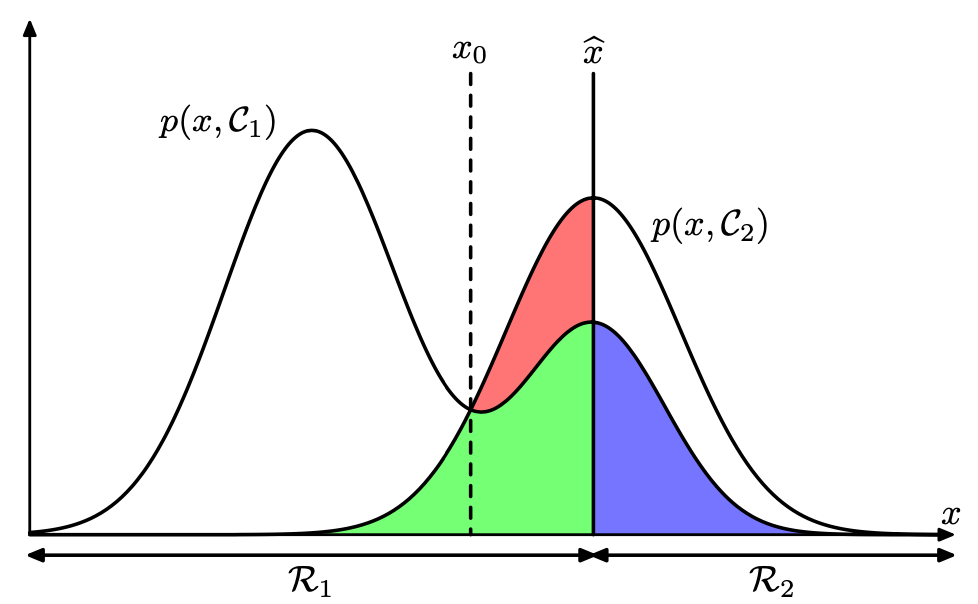
\includegraphics[height=4cm]{prml_fig_1-24.png}
                \caption{$x$ に対する,2つのクラスの同時分布 $p(x,\CC_{k})$ と決定境界 $x=\widehat{x}$ の模式図}
                \label{fig:1.24}
            \end{figure}
        \end{column}
    \end{columns}
\end{frame}

\section{期待損失の最小化}

\begin{frame}{期待損失の最小化}
    \underline{誤識別率の最小化}は,分類問題の決定を完全に解決するわけではない.
    \begin{block}{例: 医療診断問題 (再訪)}
        \begin{itemize}
            \item 癌でない患者を誤って癌と診断した場合,さらに検査が必要になる程度で済むが,癌の患者を健康であると診断した場合,治療が足りず,患者が死に至る可能性がある.
            \item 明らかに,\underline{前者の誤りを増やすことになったとしても,後者の誤りを減らすべき}.
        \end{itemize}
    \end{block}
    このような問題は,\underline{損失関数}の最小化 ($\iff$ \underline{効用関数}の最大化) によって定式化可能.
\end{frame}

\begin{frame}{期待損失の最小化}
    入力 $\bs{x}$ に対する真のクラスを $\CC_{k}$ とし,$\bs{x}$ を $\CC_{j}$ に割り当てたとしたとき,こうむる損失の値を $L_{kj}$ で表すと,それを $(k,j)$-成分とする\underline{損失行列} $L$ を考えることができる.例えば,癌の例で言えば,損失行列は以下のような形になる:
    \begin{equation}
        L = \begin{pmatrix}
            0 & 1000 \\
            1 & 0
        \end{pmatrix}. \qquad \left(k = \begin{dcases}
            1, & (\text{癌}) \\
            2 & (\text{正常})
        \end{dcases},\ j = \begin{dcases}
            1, & (\text{癌}) \\
            2 & (\text{正常})
        \end{dcases}\right)
    \end{equation}
    上記の例では,
    \begin{itemize}
        \item 正しい決定 ($k=j=1,2$) をすれば損失は無く,
        \item 健康な患者を癌と診断したとき ($k=2,j=1$) の損失を1とし,
        \item 癌の患者を健康と診断したとき ($k=1,j=2$) の損失を1000
    \end{itemize}
    としている.
\end{frame}

\begin{frame}{期待損失の最小化}
    損失関数を最小にするのが最適解だが,損失関数は\underline{未知である真のクラスに依存}.

    したがって,与えられた入力ベクトル $\bs{x}$ に対して,真のクラスの不確実性 $p(\bs{x},\CC_{k})$ を用いて,以下で計算される損失の平均 (\underline{期待損失})を最小化.
    \begin{align}
        \begin{aligned}
            \BE[L] &= \sum_{k} \sum_{j} \int_{\CR_{j}} L_{kj} p(\bs{x},\CC_{k}) d{\bs{x}} = \sum_{j} \int_{\CR_{j}} \sum_{k} L_{kj} p(\bs{x},\CC_{k}) d{\bs{x}} \\
            &= \sum_{j} \int_{\CR_{j}} \textcolor{blue}{\sum_{k} L_{kj} p(\CC_{k} \mid \bs{x})} p(\bs{x}) d{\bs{x}}.
        \end{aligned}
    \end{align}
    各 $\bs{x}$ は決定領域 $\CR_{j}$ のどれかに独立に割り当てることができる.
    
    したがって,事後クラス確率 $p(\CC_{k} \mid \bs{x})$ がわかれば,期待損失を最小化する決定規則は,新たな $\bs{x}$ を $\textcolor{blue}{\sum_{k} L_{kj} p(\CC_{k} \mid \bs{x})}$ が最小になるようなクラス $j$ に割り当てることである.
\end{frame}

\section{棄却オプション}

\begin{frame}{棄却オプション}
    クラス分類の誤差が起きるのは,入力空間の事後確率 $p(\CC_{k} \mid \bs{x})$ の最大値が1よりも大幅に小さい (同時確率 $p(\bs{x},\CC_{k})$ の値が拮抗している) ときであり,こうした領域は入力 $\bs{x}$ がどのクラスに属するかが不確か.

    応用によっては,このような場合には無理に決定をせず,クラス分類の決定を行ったものに対する誤差を小さくする方がよい (\underline{棄却オプション}).
    \begin{block}{例: 医療診断問題 (再訪)}
        \begin{itemize}
            \item 正しいクラスに分類できるかどうかがはっきりしている X 線画像は,自動的に分類するシステムを用いることが適当.
            \item 正しいクラスに分類できるかどうかが曖昧な場合については,専門家の判断にゆだねる (\underline{決定の棄却}).
        \end{itemize}
    \end{block}
\end{frame}

\begin{frame}{棄却オプション}
    \begin{columns}
        \begin{column}{0.5\textwidth}
            棄却オプションは,\underline{閾値 $\theta$} を導入し,事後確率 $p(\CC_{k} \mid \bs{x})$ の最大値が $\theta$ 以下となるような入力 $\bs{x}$ に対しては決定を棄却することによって実現可能.
            \begin{itemize}
                \item 右図では,2つの事後確率の大きい方が閾値 $\theta$ 以下の場合に入力 $x$ を棄却
            \end{itemize}
            $K$ クラス分類問題においては,閾値 $\theta$ は
            \begin{itemize}
                \item $\theta = 1 \Longrightarrow$ すべての事例が棄却
                \item $\theta < 1/K \Longrightarrow$ どの事例も棄却されない
            \end{itemize}
            となる ($\because \sum_{k} p(\CC_{k} \mid \bs{x}) = 1$).

            このように,$\theta$ の値によって棄却される事例の割合が制御される.
        \end{column}
        \begin{column}{0.5\textwidth}
            \begin{figure}
                \centering
                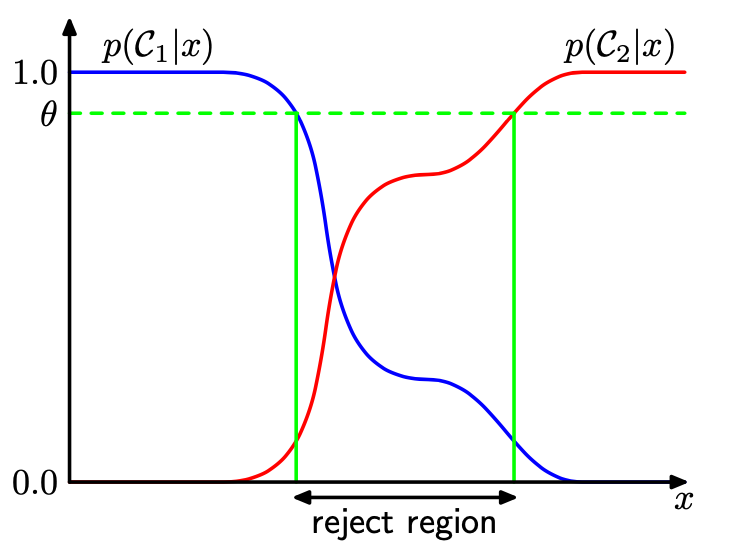
\includegraphics[height=4.5cm]{prml_fig_1-26.png}
                \caption{棄却オプションの図}
                \label{fig:1.26}
            \end{figure}
        \end{column}
    \end{columns}
\end{frame}

\begin{frame}{棄却オプション}
    棄却決定がなされたときの損失を考慮した損失行列を与えれば,期待損失を最小にするように棄却の規準を容易に一般化することができる (演習 1.24, Appendix 参照).

    \vspace{11pt}

    \begin{block}{演習 1.24 (標準) \fbox{www}}
        クラス分類問題を考え,クラス $\CC_{k}$ からの入力ベクトルをクラス $\CC_{j}$ と分類したときの損失行列を $L_{kj}$ とし,棄却オプションを選んだときの損失を $\lambda$ とする.このとき期待損失を最小とする決定規準を見つけよ.損失行列が $L_{kj} = 1 - I_{kj}$ のときは,決定規準は 1.5.3 節で議論した棄却規準に帰着されることを確かめよ.また,$\lambda$ と棄却閾値 $\theta$ にはどんな関係があるか?
    \end{block}
\end{frame}

\section{演習問題 (Appendix)}

\begin{frame}{演習問題 (Appendix)}
    \fontsize{7pt}{0cm}\selectfont
    \begin{block}{演習 1.21 (標準)}
        2つの非負の数 $a$ と $b$ があったとき,$a \le b$ なら $a \le (ab)^{1/2}$ であることを示せ.この結果を使って,2クラスの分類問題の決定領域を誤識別率が最小になるように選ぶと,この確率が
        \begin{equation}
            p(\text{誤り}) \le \int \{p(\bs{x},\CC_{1}) p(\bs{x},\CC_{2})\}^{1/2} d{\bs{x}}
        \end{equation}
        を満たすことを示せ.
    \end{block}
    (解答) $a,b \ge 0$ より,$a \le b \Longrightarrow a^{1/2} \le b^{1/2} \Longrightarrow a \le (ab)^{1/2}$ である.誤識別率が最小となる決定規則は,$p(\bs{x},\CC_{2}) \le p(\bs{x},\CC_{1})$ (resp. $p(\bs{x},\CC_{1}) \le p(\bs{x},\CC_{2})$) なる $\bs{x}$ の決定領域を $\CR_{1}$ (resp. $\CR_{2}$) と選べばよいので,
    \begin{gather}
        p(\bs{x},\CC_{2}) \le p(\bs{x},\CC_{1}) \Longrightarrow \int_{\CR_{1}} p(\bs{x}, \CC_{2}) d{\bs{x}} \le \int_{\CR_{1}} \{p(\bs{x},\CC_{1}) p(\bs{x},\CC_{2})\}^{1/2} d{\bs{x}},\\
        p(\bs{x},\CC_{1}) \le p(\bs{x},\CC_{2}) \Longrightarrow \int_{\CR_{2}} p(\bs{x}, \CC_{1}) d{\bs{x}} \le \int_{\CR_{2}} \{p(\bs{x},\CC_{1}) p(\bs{x},\CC_{2})\}^{1/2} d{\bs{x}},
    \end{gather}
    ゆえ,
    \begin{equation}
        p(\text{誤り}) = \int_{\CR_{1}} p(\bs{x}, \CC_{2}) d{\bs{x}} + \int_{\CR_{2}} p(\bs{x}, \CC_{1}) d{\bs{x}} \le \int \{p(\bs{x},\CC_{1}) p(\bs{x},\CC_{2})\}^{1/2} d{\bs{x}}. \qed
    \end{equation}
\end{frame}

\begin{frame}{演習問題 (Appendix)}
    \fontsize{7pt}{0cm}\selectfont
    \begin{block}{演習 1.22 (基本) \fbox{www}}
        $L_{kj}$ を要素とする損失行列が与えられたとき,期待リスクが最小になるのは,各 $\bs{x}$ に対し,$\sum_{k} L_{kj} p(\CC_{k} \mid \bs{x})$ を最小にするクラスを選んだときである.損失行列が $L_{kj} = 1 - I_{kj}$ で与えられたとき,これが最大事後確率のクラスを選ぶ規準に帰着されることを確かめよ.ただし,$I_{kj}$ は単位行列の成分を表す.また,この損失行列はどのように解釈できるか?
    \end{block}
    (解答) 与えられた損失行列より,
    \begin{align}
        \sum_{k} L_{kj} p(\CC_{k} \mid \bs{x}) &= \sum_{k} (1 - I_{kj}) p(\CC_{k} \mid \bs{x}) = \sum_{k} p(\CC_{k} \mid \bs{x}) - \sum_{k} I_{kj} p(\CC_{k} \mid \bs{x}) \\
        &= 1 - \sum_{k} I_{kj} p(\CC_{k} \mid \bs{x}) = 1 - p(\CC_{j} \mid \bs{x})
    \end{align}
    を得る.期待損失が最小になるのは,各 $\bs{x}$ に対し,$\sum_{k} L_{kj} p(\CC_{k} \mid \bs{x})$ を最小にするクラスを選んだときであり,これは $p(\CC_{j} \mid \bs{x})$ を最大にするクラスを選ぶことと同値であるので,最大事後確率のクラスを選ぶ規準に帰着される.また,損失行列 $L_{kj} = 1 - I_{kj}$ は対角成分が0で,対角成分以外の成分が1であるような行列なので,期待損失の最小化は,誤識別率の最小化と等価である.
\end{frame}

\begin{frame}{演習問題 (Appendix)}
    \fontsize{7pt}{0cm}\selectfont
    \begin{block}{演習 1.23 (基本)}
        一般の場合に,損失行列とクラスに対する事前確率が与えられたときに,期待損失を最小にする規準を導け.
    \end{block}
    (解答) 期待損失を最小にする規準は,損失行列 $L$ と事後確率 $p(\CC_{k} \mid \bs{x})$ を用いて,$\sum_{k} L_{kj} p(\CC_{k} \mid \bs{x})$ を最小にする規準と等価であった.ここで,事後確率 $p(\CC_{k} \mid \bs{x})$ は,ベイズの定理を用いると,クラスに対する事前確率 $p(\CC_{k})$ を用いて,
    \begin{equation}
        p(\CC_{k} \mid \bs{x}) = \frac{p(\bs{x} \mid \CC_{k}) p(\CC_{k})}{p(\bs{x})}
    \end{equation}
    と書けるので,
    \begin{equation}
        \sum_{k} L_{kj} p(\CC_{k} \mid \bs{x}) = \frac{1}{p(\bs{x})} \sum_{k} L_{kj} p(\bs{x} \mid \CC_{k}) p(\CC_{k})
    \end{equation}
    を得る.したがって,
    \begin{equation}
        \argmin_{j} \sum_{k} L_{kj} p(\CC_{k} \mid \bs{x}) = \argmin_{j} \sum_{k} L_{kj} p(\bs{x} \mid \CC_{k}) p(\CC_{k})
    \end{equation}
    となる.
\end{frame}

\begin{frame}{演習問題 (Appendix)}
    \fontsize{7pt}{0cm}\selectfont
    \begin{block}{演習 1.24 (標準) \fbox{www}}
        クラス分類問題を考え,クラス $\CC_{k}$ からの入力ベクトルをクラス $\CC_{j}$ と分類したときの損失行列を $L_{kj}$ とし,棄却オプションを選んだときの損失を $\lambda$ とする.このとき期待損失を最小とする決定規準を見つけよ.損失行列が $L_{kj} = 1 - I_{kj}$ のときは,決定規準は 1.5.3 節で議論した棄却規準に帰着されることを確かめよ.また,$\lambda$ と棄却閾値 $\theta$ にはどんな関係があるか?
    \end{block}
    (解答) 棄却を考えない場合は,期待損失の最小化は $\sum_{k} L_{kj} p(\CC_{k} \mid \bs{x})$ の最小化と等価なので,棄却オプションを考慮したときの期待損失を最小とする決定規準は,
    \begin{align}
        \min_{j} \sum_{k} L_{kj} p(\CC_{k} \mid \bs{x}) < \lambda &\Longrightarrow \text{クラス}\ \CC_{j}\ \text{を選択}, \\
        \min_{j} \sum_{k} L_{kj} p(\CC_{k} \mid \bs{x}) \ge \lambda &\Longrightarrow \text{棄却}
    \end{align}
    となる.損失行列が $L_{kj} = 1 - I_{kj}$ のときは,演習 1.22 より,期待損失の最小化は $1 - p(\CC_{j} \mid \bs{x})$ の最小化となるので,期待損失を最小とする決定規準は,
    \begin{align}
        1 - p(\CC_{j} \mid \bs{x}) < \lambda \iff p(\CC_{j} \mid \bs{x}) > 1 - \lambda &\Longrightarrow \text{クラス}\ \CC_{j}\ \text{を選択}, \\
        1 - p(\CC_{j} \mid \bs{x}) \ge \lambda \iff p(\CC_{j} \mid \bs{x}) \le 1 - \lambda &\Longrightarrow \text{棄却}
    \end{align}
    となる.したがって,棄却閾値を $\theta = 1 - \lambda$ としたとき,決定規準は 1.5.3 節で議論した棄却規準に帰着される.
\end{frame}

\end{document}